\chapter{Literature Review}

The \gls{VRP} and the \gls{CVRP} belong to the most frequently studied combinatorial
optimization problems, and are proven $NP$-hard. The goal is to minimize the total driven distance
by a fleet of vehicles, which have to start and end each tour at a central depot driving to each
customer exactly once.\footcite[cf.][p.1]{gendreau_tabu_2008} Some \gls{VRP}
instances constructed from \citeauthor{solomon_algorithms_1987}
in \citeyear{solomon_algorithms_1987} could not be solved optimally until now and the
solvation leaded rallys to solve them.\footcite[cf.][]{solomon_algorithms_1987} However,
in practical and real-world situations items can not be considered as integers of weight
and volume to check the loading, but by condidering the geometrical shape and characteristics.\footcite[cf.][p.1]{gendreau_tabu_2008}
To attain a more realistic profile of routing and loading problems, \cite{iori_exact_2004} and \cite{gendreau_tabu_2008}
solved the \gls{2L-CVRP} for the first time, considering the area of each items and allowing no stacking in
the vehicles used for delivering the items.\footcites()()[cf.][]{iori_exact_2004}[cf.][]{gendreau_tabu_2008}
This lead consequently to a more complex problem, as every route needed to be checked seperately for
a feasible loading without violating pyhsical and loading related constraints.
The applicability in practical scenarios was further increased from \cite{gendreau_tabu_2006} by defining
the \gls{3L-CVRP}, considering the stacking of items and all dimensions of items and the vehicles. The authors
also conidered a set of practical loading constraints to further enhance the applicability. \footcite[cf.][]{gendreau_tabu_2006}
The algorithms to solve the \gls{CLP} could already taken from existing literature tackling the standalone
problem.\footcite[cf.][]{pisinger_heuristics_2002} The following literature review will focus
on the \gls{CLP}, its possible constraints, algorihtms to solve it and the possibility to use solution
methods beside the classical approaches. As the \gls{CLP} is considered as a subproblem of the \gls{VRP}
in this thesis, the literature and examples refer to the \gls{3L-CVRP} and each problem should not be
considered solely.


\section{Container Loading Problem}
\label{sec:clp_definition}

The placement and assignment of items to larger, mostly rectangular
containers, is a well known problem in logistics and operations research, as the
potential of cost savings and efficiency gains is substantial by reducing the number
of needed containers or by fulfilling customer needs. The \gls{CLP} covers a broad range of real-world applications,
such as loading cargo, optimizing warehouse storage and packing of pallets or cardboard boxes.
Generally it is differentiated in \textit{input minimization},
where the number of needed containers is minimized, and \textit{output maximization} problems,
where the value of the associated items is maximized. The \gls{BPP} is the generalized problem type of the \gls{CLP}
and belongs to \textit{input minimization} problems, whereas the knapsack problem to \textit{output maximization}. Apart from the expected outcome of the optimization,
the characterics of the items and containers is crucial for the problem definition. Items can be either
homogeneous or heterogeneous in size and shape. Furthermore, they can be classified as weakly or strongly
homogeneous or heterogeneous, depending on the degree of similarity among them. The container is
defined as a recangular volume with a fixed size and shape, where the items have to be placed in.
Other, non rectangular, shapes are seldomly considered in the literature, as the practical relevance is
limited. Multiple containers of homogeneous or heterogeneous sizes are used when the volume and weight
of the cargo require it.\footcite[cf.][pp. 1--2]{bortfeldt_constraints_2013}
According to \textcite{bischoff_issues_1995}, the mere placement of items in containers is insufficient
if practical requirements are not fulfilled as it lacks applicability. \footcite[cf.][pp. 1--2]{bischoff_issues_1995}
\textcite{bortfeldt_constraints_2013} systematically categorized all constraints emphasized in \gls{CLP} research
into five categories, which are presented in the following. They also distinguish between hard and soft constraints,
where hard constraints must be strictly satisfied, while soft constraints may be violated
to some extent.\footcite[cf.][p. 2]{bortfeldt_constraints_2013}  Figure~\ref{fig:solution-visualization}
visualizes a possible 3D packing with different constraints applied.

\begin{figure}[ht]
    \centering
    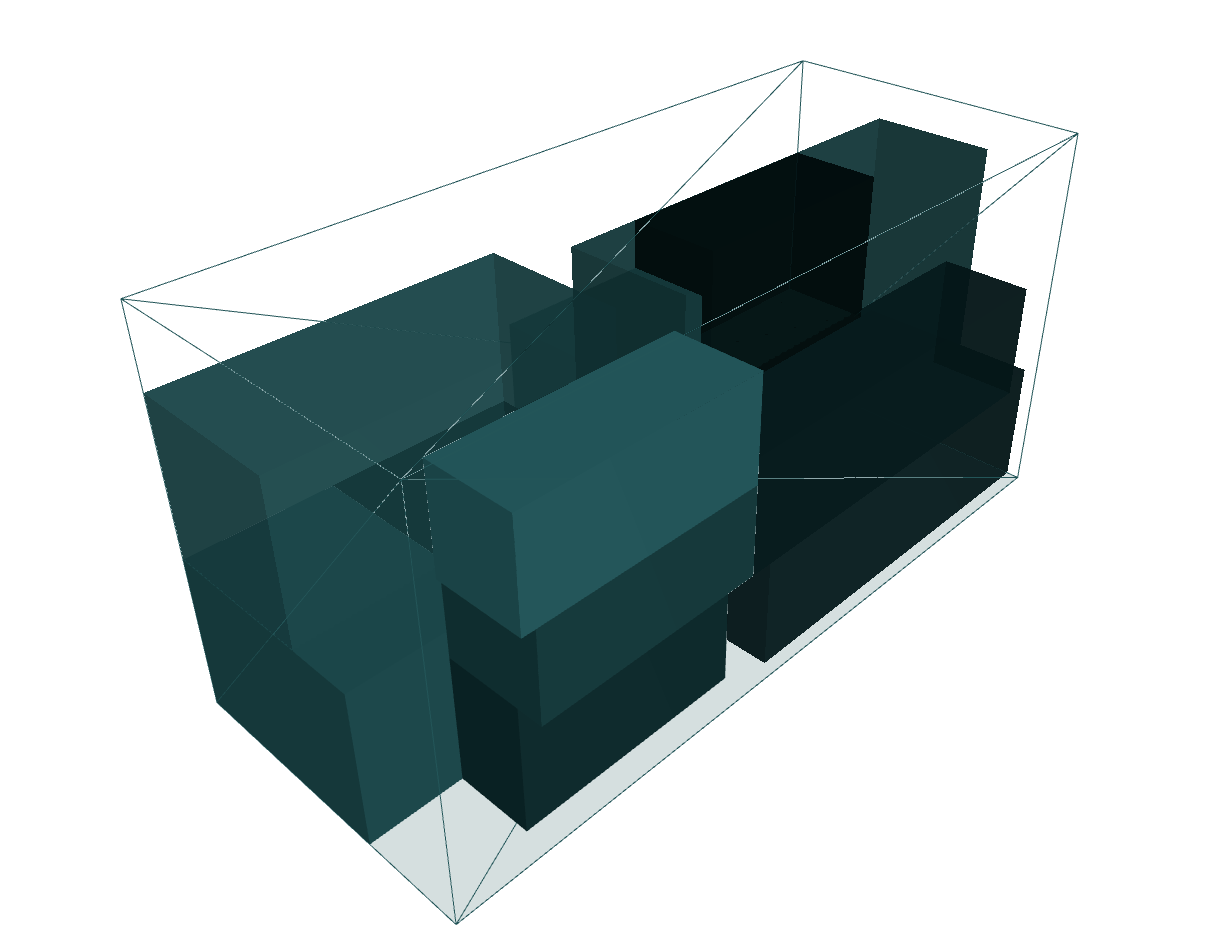
\includegraphics[width=6.3cm]{pictures/3l_cvrp_example.png}
    \caption[Visualized 3D packing with packing constraints.]{3D Packing with geometry, orthogonality and support area constraints.\footnotemark}.
    \footnotetext{CLP Visualizer from \textcite{tamke_branch-and-cut_2024}.}
    \label{fig:solution-visualization}
\end{figure}

\subsubsection{Container related constraints}
These constraints summarize all physical barriers of the container. The \textit{load capacity} limits the aggregated
mass of all items in the container. The distribution of the weight (\textit{load balance})
plays an important role for safety reasons, as the cargo must not move during the transport and the container
must not tip over and is defined by the maximum weight difference between the left and right half of the container.
When the containers are transported by trucks, uneven \textit{axle weight} distribution can cause severe
consequences and need to be avoided for practicability by loading the cargo axle-friendly. \footcite[cf.][pp. 849--850]{krebs_advanced_2021}

\subsubsection{Item related constraints}
Item related constraints define the properties of the item, which are relevant
for the packing. When the container capacity is limited (output maximization),
the \textit{loading priority} constraint defines the priority among possible
item candidates. The \textit{orientation} constraint restricts how an item can be rotated.
There are several types of rotation, each defined by the axis around which the item rotates.
The most common is the \textit{z-rotation}, where rotation is only allowed around the vertical axis.
When 3D packing is considered, stacking of items is allowed in comparison to 2D packing, when all
items are placed on the container floor. Two main approaches exist, when stacking is considered.
The \textit{fragility} constraint differentiates between fragile and non-fragile items,
allowing only non-fragile items to be stacked on non-fragile items. Figure \ref{fig:stacking_comparison} showcases
this definition. The other approach defines an individual \textit{\gls{LBS}} for each
item stating how much pressure the box can tolerate, and which items can be stacked. \footcite[cf.][pp. 847--848]{krebs_advanced_2021}

\begin{figure}[htbp]
    \centering
    \small
    % First TikZ picture
    \begin{subfigure}[b]{0.45\textwidth}
        \centering
        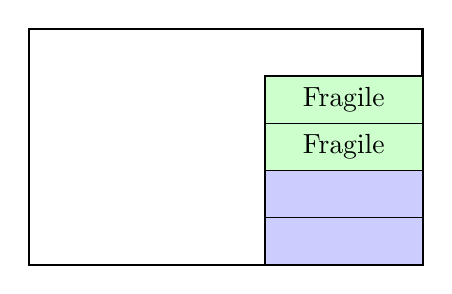
\begin{tikzpicture}
            % Draw the container
            \draw[thick] (0,0) rectangle (5,3);

            % Draw the three items inside
            \draw[fill=blue!20] (3,0) rectangle (5,0.6);
            \node at (4, 0.3) {};

            \draw[fill=blue!20] (3,0.6) rectangle (5,1.2);
            \node at (4, 0.9) {};

            \draw[fill=green!20] (3,1.2) rectangle (5, 1.8);
            \node at (4, 1.5) {Fragile};

            \draw[fill=green!20] (3,1.8) rectangle (5, 2.4);
            \node at (4, 2.1) {Fragile};

        \end{tikzpicture}
        \caption{Feasible stacking of items.}
    \end{subfigure}
    \hfill
    % Second TikZ picture
    \begin{subfigure}[b]{0.45\textwidth}
        \centering
        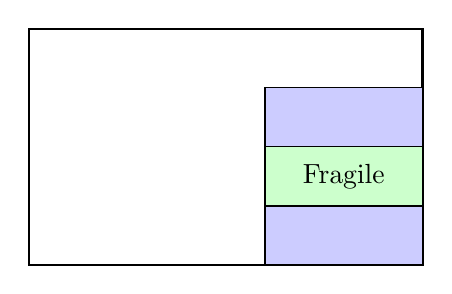
\begin{tikzpicture}
            \draw[thick] (0,0) rectangle (5,3);

            % Draw the three items inside
            \draw[fill=blue!20] (3,0) rectangle (5,0.75);
            \node at (4, 0.5) {};

            \draw[fill=green!20] (3,0.75) rectangle (5,1.5);
            \node at (4, 1.125) {Fragile};

            \draw[fill=blue!20] (3,1.5) rectangle (5, 2.25);
            \node at (4, 1.875) {};
        \end{tikzpicture}
        \caption{Infeasible stacking of items.}
    \end{subfigure}
    \caption[Visualization of fragility constraint.]{Comparison of fragile stacking (side view).}
    \label{fig:stacking_comparison}
\end{figure}


\subsubsection{Cargo-Related Constraints}
In contrast to item-related constraints, cargo-related constraints apply to
the entire cargo or to specific subsets of it. The \textit{complete-shipment} constraint
requires that all items within a shipment must either be loaded into the same
container or be left behind entirely. This constraint is important
when container capacity is limited (output maximization) and items
cannot be split. The \textit{allocation} constraint serves a similar purpose,
including the \textit{connectivity} constraint, which mandates that
certain items must be loaded into the same container, and the
\textit{separation} constraint, which requires specific items to
be distributed across different containers. For example, kitchen
shipments, comprising multiple packages, should be delivered together
to enable efficient installation. Conversely, items such as perfume and fresh
vegetables should be shipped separately due to incompatibility.

\subsubsection{Positioning constraints}

Positioning constraints determine, if items must be placed at
absolute locations or relative to other items. Absolute positioning is
typically based on item characteristics such as size, weight, or
content (e.g., bulky or hazardous items placed near the container door for accessibility) or
they may universally apply to all items, as the \textit{geometry} and
\textit{orthogonality} constraints. These constraints define that items are not allowed to overlap
and must be placed orhogonally to the container walls respectively.
Relative positioning requires items to be placed either close together as a \textit{group} or
\textit{separated} from each other.
The multi-drop constraint combines absolute and relative positioning requirements for items
destined for different delivery locations. The goal is to minimize reloading efforts by grouping items
by destination, arranging these groups in the delivery sequence, and applying either a \textit{\gls{LIFO}}
or sequential loading policy to ensure efficient unloading without having to move unrelated items.
Variations of the \gls{LIFO} constraint account for manual unloading (\textit{\gls{MLIFO}}) or unloading based on the
maximum allowable distance reachable from the unloading point (\textit{reachability}).

\subsubsection{Load-related constraints}

The \textit{stability} constraint is defined as one of the most critical constraints
in the \gls{CLP}, as it directly impacts the safety of both the cargo and the personnel involved.
First, a distinction must be made between \textit{horizontal} and \textit{vertical} stability.
Horizontal stability is achieved when items are securely connected to the
container walls or to other items, preventing lateral movement. Vertical
stability, on the other hand, is defined in various ways throughout the
literature. A common approach to assessing vertical stability is through the concept of the \textit{support
    area}, the portion of an item's base that rests on the surface below. Stability is typically
considered sufficient when the support area covers $75\%$ to $100\%$ of the item’s base. \footcite[cf.][p. 344]{gendreau_tabu_2006} However,
this may still result in unstable configurations if the center of gravity falls outside the
support area of the underlying layers, potentially causing the cargo to tilt. To improve practical stability,
a more reliable definition of vertical stability requires a minimum support area for all items below,
referred to as \textit{robust stability}.\footcite[cf.][p. 1140]{ceschia_local_2013} This comparison is illustrated in Figure~\ref{fig:vertical_stability_comparison}.
Additionally, it is crucial to ensure that the load remains stable even after partial unloading.
In addition, complexity constraints refer to specialized
requirements that are beyond standard packing rules. These include, for example, compatibility with automated or robot-assisted packing systems.
\begin{figure}[htbp]
    \centering
    \footnotesize
    % First TikZ picture
    \begin{subfigure}[b]{0.45\textwidth}
        \centering
        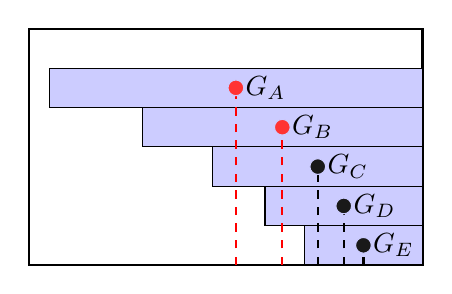
\begin{tikzpicture}
            % Draw the container
            \draw[thick] (0,0) rectangle (5,3);

            % Draw the three items inside
            % Draw the five items and their labels
            \draw[fill=blue!20] (3.5,0) rectangle (5,0.5);
            \draw[thick,dashed,black] (4.25,0) -- (4.25,0.25);  % <---
            \draw[fill = black!90, draw = blue!20] (4.25,0.25) circle (0.1);
            \node[anchor=west] at (4.25,0.25) {$G_E$};

            \draw[fill=blue!20] (3,0.5) rectangle (5,1);
            \draw[thick,dashed,black] (4,0) -- (4,0.75);  % <---
            \draw[fill = black!90, draw = blue!20] (4,0.75) circle (0.1);
            \node[anchor=west] at (4,0.75) {$G_D$};

            \draw[fill=blue!20] (2.33,1) rectangle (5,1.5);
            \draw[thick,dashed,black] (3.67,0) -- (3.67,1.25);  % <---
            \draw[fill = black!90, draw = blue!20] (3.67,1.25) circle (0.1);
            \node[anchor=west] at (3.67,1.25) {$G_C$};

            \draw[fill=blue!20] (1.44,1.5) rectangle (5,2);
            \draw[thick,dashed,red] (3.22,0) -- (3.22,1.75);  % <---
            \draw[fill=red!80, draw = blue!20] (3.22,1.75) circle (0.1);
            \node[anchor=west] at (3.22,1.75) {$G_B$};

            \draw[fill=blue!20] (0.26,2) rectangle (5,2.5);
            \draw[thick,dashed,red] (2.63,0) -- (2.63,2.25);  % <---
            \draw[fill=red!80, draw = blue!20] (2.63,2.25) circle (0.1);
            \node[anchor=west] at (2.63,2.25){$G_A$};


            %\node at (4, 1.875) {Fragile};
            %\node[anchor = west,align=center] at (2.9,2.5) {\small Center of \\  balance};

        \end{tikzpicture}
        \caption{Feasible, but unrobust, stacking with 75\% support area.}
    \end{subfigure}
    \hfill
    % Second TikZ picture
    \begin{subfigure}[b]{0.45\textwidth}
        \centering
        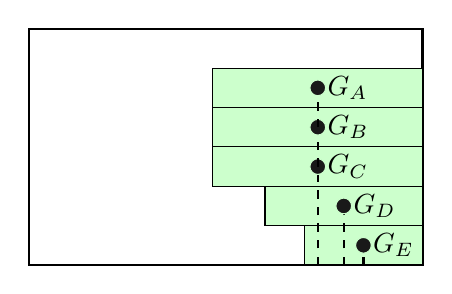
\begin{tikzpicture}
            % Draw the container
            \draw[thick] (0,0) rectangle (5,3);
            % Draw the three items inside
            % Draw the five items and their labels
            \draw[fill=green!20] (3.5,0) rectangle (5,0.5);
            \draw[thick,dashed,black] (4.25,0) -- (4.25,0.25);  % <---
            \draw[fill = black!90, draw = green!20] (4.25,0.25) circle (0.1);
            \node[anchor=west] at (4.25,0.25) {$G_E$};

            \draw[fill=green!20] (3,0.5) rectangle (5,1);
            \draw[thick,dashed,black] (4,0) -- (4,0.75);  % <---
            \draw[fill = black!90, draw = green!20] (4,0.75) circle (0.1);
            \node[anchor=west] at (4,0.75) {$G_D$};

            \draw[fill=green!20] (2.33,1) rectangle (5,1.5);
            \draw[thick,dashed,black] (3.67,0) -- (3.67,1.25);  % <---
            \draw[fill = black!90, draw = green!20] (3.67,1.25) circle (0.1);
            \node[anchor=west] at (3.67,1.25) {$G_C$};

            \draw[fill=green!20] (2.33,1.5) rectangle (5,2);
            \draw[thick,dashed,black] (3.67,1.25) -- (3.67,1.75);  % <---
            \draw[fill = black!90, draw = green!20] (3.67,1.75) circle (0.1);
            \node[anchor=west] at (3.67,1.75) {$G_B$};

            \draw[fill=green!20] (2.33,2) rectangle (5,2.5);
            \draw[thick,dashed,black] (3.67,1.75) -- (3.67,2.25);  % <---
            \draw[fill = black!90, draw = green!20] (3.67,2.25) circle (0.1);
            \node[anchor=west] at (3.67,2.25) {$G_A$};


            %\node at (4, 1.875) {Fragile};
            %\node[anchor = west,align=center] at (2.9,2.5) {\small Center of \\  balance};

        \end{tikzpicture}
        \caption{Feasible and robust stacking regarding 75\% support area.}
    \end{subfigure}
    \caption[Comparison of different vertical stability constraints.]{Comparison of different vertical stability constraints \\ with G = Center of Gravity (container side view). \footnotemark}
    \footnotetext{Own figures based on \textcite[p. 845]{krebs_advanced_2021}.}
    \label{fig:vertical_stability_comparison}
\end{figure}


\cite{gendreau_tabu_2006} showed, that the conisdered set of constraints for the \gls{CLP} significantly
changes the complexity and solution quality for the \gls{3L-CVRP}. In average, the solutions are $15.87\%$ better
costwise and the CPU-time was significantly lower, when no additional constraints are considered.\footcite[cf.][p.348]{gendreau_tabu_2006} The loading constraints
are therefore crucial for pre-determining the time for computation as well as the complexity and the applicability
of the solutions, which is very important. The following section highlights classical solution approaches
of the \gls{CLP} in \gls{3L-CVRP} scenarios.


\section{Classical Solution Approaches}
\label{sec:classical_solution_approaches}
The \gls{CLP} is a NP-hard combinatorial problem. \footcite[cf.][p. 11]{bortfeldt_constraints_2013}
Consequently, heuristics and metaheuristics were the dominating tools
in the early stages of this research field.\footcite[cf.][]{pisinger_heuristics_2002} The variety of methods
and their solution quality for solving the 2D \gls{CLP} developed in recent years. \footcite[cf.][p. 23]{iori_exact_2021}
When the \gls{CLP} is considered as subproblem of the \gls{VRP} the focus shifts from finding optimal
packing solutions to guaranteeing feasibility for the loading of one cost-wise optimal route. Therefore
speed and reliability are the main motivations for a good solution algorihtm.
The variety of 3D algorithms, especially for exact methods, is in comparison limited, as
\textcite{zhao_comparative_2016} elaborated in their survey. The following Figure~\ref{fig:solution_methods_overview}
presents this overview of the solution methods for the 3D \gls{CLP}.\footcite[cf.][]{zhao_comparative_2016}
It is divided in three categories constructive heuristics, metaheuristics
and exact methods. Hybrid methods and improvement heuristics are not explicitly shown in the figure,
as the former combines components from multiple categories, while the latter is subsumed within
metaheuristics. It needs to be noted, that Heuristics can fail to identify a feasible solution as such
one in comparison to exact algorihtms, but are computationally very lightweight approaches.
The depicted solution methods are described in the following.

\begin{figure}[htbp]
    \centering
    \resizebox{0.55\linewidth}{!}
    {
        \begin{tikzpicture}[grow cyclic, text width=2.7cm, align=flush center,
                level 1/.style={level distance=3.5cm,sibling angle=120},
                level 2/.style={level distance=3.5cm,sibling angle=50}
            ]

            \node {Solution Techniques \gls{CLP}}
            child { node {Metaheuristics}
                    child { node {Simulated Annealing}
                            child{node{One Stage Local Search Solver}}}
                    child { node {Tabu Search}}
                    child { node {Evolutionary Algorithm}}
                    child { node {Augmented extreme point-based heuristic}}
                }
            child { node {Exact \\ Methods}
                    child { node {Constraint Programming}}
                    child { node {Mixed-integer programming}}
                }
            child { node {Constructive Heuristics}
                    child { node {Layer/ Wall/ Tower Building}}
                    child { node {Corner Point Algorithms}
                            child{node{Minimize Waste Area}}}
                    child { node {Bottom-Left-Fill}
                            child{node{Deepest-Bottom-Left-Fill}}}
                    child { node {Maximum Touching Perimeter}
                            child{node{Maximum Touching Area}}}
                    child { node {Tree Search Algorithm}}
                }
            ;

        \end{tikzpicture}
    }
    \caption{Overview of solution methods for the container loading problem.}
    \label{fig:solution_methods_overview}
\end{figure}



\subsubsection{Constructive Heuristics}
For obtaining an initial feasible solution, two primary strategies are commonly
used depending on the heterogeneity of the items. In cases where the items are weakly homogeneous,
the problem dimensionality is reduced from 3D to 2D by constructing either
\textit{walls} or \textit{layers} of similarly sized items. These structures fill one
dimension of the container, typically either length and height or width and length, thereby
simplifying the remaining problem space. Moreover, when the layers or walls have
equal dimensions approximately, horizontal and vertical stability constraints are met.
Beyond these two dominant approaches, several adaptations exist to address item heterogeneity.
For example, \textcite{gehring_genetic_1997} propose the construction of item
\textit{towers}, in which boxes are stacked on top of other items so that the base of the box is covered completely
by the box below it. This effectively reduces the dimensions from 3D to a 2D floor space arrangement,
similar to the \gls{PLP}.\footcite[cf.][pp. 402--406]{gehring_genetic_1997}
In the integrated approach for solving the subproblem of the \gls{2L-CVRP} resp. \gls{3L-CVRP}
the most common heuristics are variations of the \textit{\Gls{BLF}}
and the \textit{\Gls{MTP}} algorithm. The first algorithm describes the order, where
every consecutive item is tried to be placed as close to the bottom left corner of the vehicle.
When constraints as \gls{LIFO} are considered, \cite{iori_exact_2007} utilized a \textit{contour} line
to identify the last possibble placement of each item on the floor. The second algorithm is introduced by
\cite{zachariadis_guided_2009} and inserts the next item reagrding the maximum total length of the item which is connected
to other items and to the container wall (An alternative is also proposed, where walls are excluded).\footcite[cf.][p.732f]{zachariadis_guided_2009}
For the three-dimensional problem the heuristics from the \gls{2L-CVRP} were adapted to be also suiting
when considering stacking and multiple layers of items. In \cite{gendreau_tabu_2006}, the Bottom-Left-Algorithm
was adapted, that the items were to the bottom (first priority) and to the left (second priority) of the cargo space.
and the maximum touching perimeter is adapted by not only considering the maximum
perimeter of each item connecting with other items and the container walls, but the whole three-dimensional
surface (touching area algorithm). \footcite[cf.][p. 345]{gendreau_tabu_2006} In the work from \cite{tao_effective_2015} a corner point method
was introduced, which aims to minimize the waste area (unused loading capacities, blocked space) by
defining for each item all possible corner points, where the item could be placed in all possible
orientations.\footcite[cf.][pp. 130-132]{tao_effective_2015} The \gls{DBLF} algorithm
is an adaption of the \gls{BLF} Algorithm and was integrated in the \gls{3L-CVRP} from \cite{krebs_advanced_2021}.
The core adaption is, that the first priority for placing any item is as far as possible in the back of the cargo
leading to a more dense packing.\footcite[cf.][pp 8-9]{krebs_axle_2021}
Even though constructive heuristics are quite simple, they are still widely used because of their simplicity and efficiency to obtain fast solutions.
\footcite[cf.][pp. 11--13]{tamke_branch-and-cut_2024}

\subsubsection{Metaheuristics}
Once an initial solution is found, metaheuristics or improvement heuristics can be applied
to improve it. Therefore a solution representation, such as a permutation of items, is required
to conduct changes of the current solution. \gls{GA}s were
used to either improve the walls, towers or layers found by the constructive heuristics
or by improving the quality of the permutation of all items. \footcite[cf.][]{gehring_genetic_1997}
\gls{TS} is a widely used approach for \gls{BPP} and \gls{CLP}. It is based on
the idea of iteratively improving a solution by exploring its neighborhood and simultaneously
storing certain moves or complete solutions in a tabu list to avoid back-cycling to
previous solutions, feasible or infeasible ones. \footcite[cf.][pp. 344--345]{gendreau_tabu_2006}
\gls{SA} has rarely been used as a standalone metaheuristic in the context of \gls{CLP}, but is often
combined with other approaches to benefit the temperature dependent acceptance criterion of
solutions. As \gls{SA} mimics the cooling curve from hot metal, at the beginning of the algorithm the probability
to accept worse solutions is higher as the algorithm cooling precedes, shifting from diversification to
intensification. This helps the algorithm to escape local optima
early in the search and gradually transition into more focused phase. \cite{ceschia_local_2013} suggests
the usage of a one-stage \gls{LS} solver, which is directly improving the order of the items being
loaded on the vehicles instead of the customers. By combining a \gls{LNS} as
well as \gls{SA} the solutions are allowed to be infeasible durign the procedure and become repaired during
the iterations and several loading heuristics are being selected from. This was the first work to
solve the loading and routing completely integrated on item level. \footcite[cf.][pp. 1142-1145]{ceschia_local_2013}
\cite{tamke_branch-and-cut_2024} implemented a \textit{augmented extreme point-based metaheuristic}
to speed-up the exact \gls{3L-CVRP} algorithm by reducing calls of the \gls{CP} solver, whenever the heuristic
found a feasibile solution. This metaheuristic is based on the extreme point heuristic from \cite{zhang_evolutionary_2015},
but adds several diversification and intensification elements as perturbation and \gls{LS} to find
loading solutions feasible and quality assuring for their exact algorithm.\footcite[cf.][pp. 11-13]{tamke_branch-and-cut_2024}
In their work \cite{kucuk_constraint_2022} propose a hybrid approach for solving \gls{3L-CVRP} solving the
masterproblem \gls{VRP} optimally with an exact solver and using an \gls{EA}
to solve the \gls{CLP}. The approach is very similar to using a \gls{GA}, but \gls{EA}
do have a better structural design flexibility.\footcite[cf.][pp. 5--8]{kucuk_constraint_2022}

\subsubsection{Exact Algorithms}
Retrieving optimal solutions for the \gls{CLP} is computationally challenging in comparison
to finding good solutions with heuristics. The main difficulty is to represent packing
patterns and the constraints introduced in Section~\ref{sec:clp_definition} in a mathematical way.
Two prominent methods exist for modeling the \gls{CLP}. The first one is \gls{LP}, which can be
formulated in two primary ways. One approach defines each possible packing pattern as
a variable. \footcite[cf.][pp. 29--30]{zhu_prototype_2012} The second approach models
the placement of items using discrete coordinate variables. Each placement of an item
is defined by the cartesian coordinate tupel of the depeest, leftest and lowest corner point of
the item.\footcites[cf.][pp. 649-653]{junqueira_optimization_2013}[cf.][pp. 4--8]{moura_integrated_2009}
Both formulations can benefit from enhancements such as branch-and-price or branch-and-cut
methods, which reduce the search space and improve solution time.
The second main method is \gls{CP}, which offers a flexible alternative for handling
complex constraints, where the focus is to find feasible solutions primarily and
not fulfilling an optimization criterion directly. \cite{tamke_branch-and-cut_2024} used a \gls{CP} Solver
to solve the loading of single tours and were the first authors to introduce an exact algorithm
considering many looding constraints. \footcite[cf.][pp. 7--11]{tamke_branch-and-cut_2024}
A similar approach was conducted by \cite{hokama_branch-and-cut_2016}, which extended their
branch-and-cut approach, to be able to insolve three-dimensional packings as well.
They also used a \gls{CP} model for feasibility checks, but considered less loading constraints. \footcite[cf.][]{hokama_branch-and-cut_2016}
\textcite{iori_exact_2021} states, that
\gls{CP} improved the results of 2D \gls{CLP} problems significantly and is a promising
field of future research.\footcite[cf.][p. 23]{iori_exact_2021}

\footcite[cf.][]{hokama_branch-and-cut_2016}

\begin{comment}
Gibt es denn abseits von Kücük Exakte Algorithmen oder wird nur
Spaltengenerierung als Teil einer Heuristik vorgestellt?
\end{comment}

\parbreak

In general exact methods are not capable of solving large instances with practical relevance
in reasonable computation time. In their study to solve the Gendreau Instances exact with all loading constraints,
\cite{tamke_branch-and-cut_2024} could solve instances up to 41 customers with an optimality
gap below $5 \%$. However the results, can be used to understand the structure
of optimal solutions to provide lower bounds and guidance for the development of future
heuristics. A possible approach to improving
the performance of exact algorithms is the use of speed-ups. Depending on the complexity of
the conidered loading constraints, the routing or the loading feasibiltiy check is the computational
bottleneck in finding the optimal solution. \cite{tamke_branch-and-cut_2024} attempted to add
stronger cuts to the solution and implementing a Set Partitioning Heuristic as well as a
heuristic to speed up the feasibility checks on the loading. At a total run time of 8 hours the feasibility
checks were the slow down effect as for 3 instances these checks made up more than $50\%$ of the total run time. \footcite[cf.][p. 2]{tamke_branch-and-cut_2024}
Instead of using algorithmic speed-ups, some modern approaches in the loading and routing field tried
to instrumentalize pretrained \gls{ML} models for boosting the solving progress.
These models can substitute parts of the algorithm's computation time by predicting solution
feasibility or by quickly identifying good solutions, thereby reducing the computational effort
in iterative procedures, as will be further discussed in the next section.

\section{Motivation for Feasibility Prediction}
\label{sec:motivation_feasibility_prediction}
This section explores how \gls{ML} algorithms can enhance \gls{3L-CVRP} solution strategies,
highlighting both benefits and limitations. Papers, which use predictive methods to accelerate the computation time
will be analyzed. It is important to note that
several \gls{ML} approaches address the \textit{on-line} \gls{BPP}, where the optimal placement
of individual items, arriving sequentially, must be determined.\footcite[cf.][p. 1]{ali_-line_2022}
Since this work focuses on the \textit{off-line} \gls{BPP}, where a placement for all items is determined
simultaneously, on-line approaches are not further considered.
The usage of classifiers is promising to complement exisiting algorithms, as shown in the following.


\subsubsection{Feasibility Classifier of the \cgls{2L-CVRP}}
As the number of customers is increasing, the number of routes is growing exponentially and the number of
possible loading combinations even more. As shown in the exact \gls{3L-CVRP} algorithm from \cite{tamke_branch-and-cut_2024}
the feasibility checks of the loading are at a specific instance size the limiting computational factor in
exploring the exact branch-and-bound tree for the optimal solution. \footcite[cf.][p.22]{tamke_branch-and-cut_2024}
Instead of using a complementary heuristic for boosting the feasibility checks,
\textcite{zhang_learning-based_2022} used a binary classifier to predict the feasibility of the
loading of single tours to reduce the overall computation time in their exact branch-and-price \gls{2L-CVRP}
algorithm. The classifier labeled each loading of a respective route in infeasible or feasible, which
reduced the frequency of calling the exact feasibility checker by $87.22\%$ and reduced the CPU time by $54.12\%$ on average.
The exact \gls{SP} algorithm is called then only when single routes were labeled as infeasible to avoid
omitting feasible tours or before complete solutions are accepted as new \gls{LB} or \gls{UB} of the
exact branch-and-price prodecure to avoid false-positive values. To train the binary classifying model
50,000 tours were obtained by saving them, while running the underlying column generation
algorithm with just the exact feasibility checker. In their paper, they have chosen a \gls{FFNN} model, a special type of \gls{ANN} model,
from the PyTorch Library and compared it with a \gls{LR} model. In this comparison the \gls{FFNN} model had
an accuracy of at most $94.1\%$ and the \gls{LR} model had a significantly smaller value.
The models were trained in many epochs using the \textit{Mini-Batch Gradient Descent Algorithm}. The prediction and training
of the loading of tours is based on 17 hand-crafted features capturing geometric
and spatial characteristics of the packing problem. These include the ratio of the total item area
to the container floor area, as well as the mean, standard deviation, minimum, and maximum of
the following four indicators:
\begin{itemize}
    \item[1.] The ratio of item width to item height.
    \item[2.] The ratio of item width to the container width.
    \item[3.] The ratio of item height to the container height.
    \item[4.] The ratio of each item’s area to the total container area.
\end{itemize}

Even though, the results are very positive, some simplifications regarding the loading were assumed. Stacking
of items is prohibited, and only the area of the items is important, reducing the number of items significantly.
Additionally, practical loading constraints as \gls{LIFO} to avoid unloading of the items or horizontal stability
were not explicitly considered, reducing the problem complexity and therefore increasing the possibility to describe
the laoding pattern with numerical features. \footcite[cf.][]{zhang_learning-based_2022}

\subsubsection{Pallet Size Classifier for the \gls{PLP}}
Another use case for \gls{ML} in packing problems is presented by \textcite{aylak_application_2021},
who focus on selecting the optimal pallet size in the context of the \gls{PLP}. Here a number of fixed items
need to be placed on pallets with fixed weight, length and height dimensions, optimizing the volume utilization
generating subsequently stability and minimizing the number of pallets needed. Based on real-life data
three candidate pallet sizes were considered and the best packing pattern must be found for each packing
configuration defined by the number of boxes and their uniform size. Therefore, multiple packing heuristics were applied to
generate feasible packing patterns and identify the best-performing. These are used as labels for several
\gls{ML} models, which were trained to predict the optimal pallet size based on four input features: the box
dimensions \{x,y,z\} and the demand quantity. Compared to the purely heuristic approach, the classifier-based
determination achieved a volume utilization improvement of $6.7\%$ and significantly reduced computation time.
However, the study did not consider additional constraints such as weight limits, stacking rules, or stability.\footcite[cf.][pp. 12--14]{aylak_application_2021}

\subsubsection{Reinforcement Learning for th \gls{3L-CVRP}}
Another approach was chosen by \cite{schoepf_using_2024}, arguing that single heuristics are too domain and use
case specifc and proposing the usage of a \gls{RL} model for both the routing and loading. \gls{RL} is accounting
to unsupervised \gls{ML} models, where an agent selects one of several options on every stage, relying on random choices or
on past actions, interpreting the feedback of this choice again. The goal of the agent is to learn independently
the patterns which lead to the highest reward resp. the lowest loss. Even though the authors could not beat
the best cost results from heuristics solving the gendreau benchmark, they had very low computation times and
a linear increase in computational effort for bigger instances. This founds the motivation to propose, that \gls{RL}
models will be able to solve \gls{3L-CVRP} problems of big instances better and easier than currently dominating
algorithms. \footcite[cf.][]{schoepf_using_2024}

\parbreak

These examples demonstrate that \gls{ML} models can be successfully integrated into existing \gls{3L-CVRP}
algorithms to reduce computation time and overall complexity, provided the model is well trained.
However, training such a model is often time-consuming, and the practicality of both training and
integrating it must be carefully evaluated on a case-by-case basis.
In the two examples presented, the number of loading constraints was relatively small, allowing the classifier
to be trained with a limited set of features. When more complex constraints are introduced, such as
\gls{LIFO} unloading rules or item fragility, the construction of numerical features that accurately
represent these constraints becomes significantly more challenging.
Moreover, results achieved by simple classifiers often lack practical relevance, since real-world
scenarios, such as loading large containers or trucks, inevitably involve multiple constraints that
must be taken into account. \footcite[cf.][pp. 1--2]{bischoff_issues_1995} Therefore, the development of a classifier is not only demanding but also
requires careful consideration to ensure a favorable cost-benefit ratio.
A particularly promising and practically relevant application is the prediction of the feasibility of single tours for the
\gls{3L-CVRP} with constraints, an extension of the \gls{2L-CVRP} example discussed earlier. In the
\gls{3L-CVRP}, a large number of routes must be evaluated to identify those that minimize the total
distance traveled by all vehicles. While the packing of requested items does not need to satisfy
optimization criteria, it must still be feasible under the given \gls{CLP} constraints.\footcite[cf.][]{tamke_branch-and-cut_2024}
As discussed in Chapter~\ref{sec:classical_solution_approaches}, the verification of
packing feasibility for each individual route is computationally expensive.
Here, classifiers can significantly boost performance of existing exact algorithms by rapidly predicting the feasibility of the route. The
exact packing solution is then only computed for the final solution candidates or before an infeasible classified solution
is discarded to avoid incorrect eliminations, as presented above.
To facilitate this approach, a comparison of various published \gls{3L-CVRP} datasets will be conducted
to compare and identify the most appropriate dataset for training a binary feasibility classifier.


\section{Literature Overview}
The presented literature is grouped in three groups, namely metaheuristics, exact approaches and blended
approaches, in Table~\ref{tab:literature overview}. As the emphasis is lying on the distinction
if the laoding of one route is feasible or not, the routing algorithms were not presented so far.
The overview table gives here an impression into the methods and algorithms used for
optimizing the master problem, the \gls{VRP}. Most heuristic methods rely on \gls{LS} neighborhoods,
which are embedded in a metaheuristic, as \gls{SA}, \gls{LNS} or \gls{TS}. To group the approaches
further different sets of loading constraints are defined by the auhor are summarized in Table~\ref{tab:constraint_sets}.
When analyzing the three approach groups it is apparent, that the metaheuristic approaches considered
the most loading constraints. This is a consequence of the more complex definitions needed for
exact methods or the \gls{ML} approaches and the computational time surplus. Furthermore, when
the \gls{3L-CVRP} is tackled instead of the \gls{2L-CVRP}, more loading constraints, than just sequence
can be considered as the laoding gets much more complex due to the added dimension.

\begin{table}[ht]\footnotesize
    \centering
    \setlength{\tabcolsep}{3pt}         % tighten intercolumn space (default ~6pt)
    \renewcommand{\arraystretch}{1.2}   % a touch more row height

    \begin{tabular}{@{}
            P{0.25\textwidth} % Author
            P{0.15\textwidth} % Set Symbol
            P{0.50\textwidth} % Problem
            @{}}
        \toprule
        \textbf{Author}            & \textbf{Set Symbol} & \textbf{Constraints}                                                                   \\
        \midrule
        \cite{gendreau_tabu_2006}  & $\mathcal{G}$       & z-Rotation, Fragility, LIFO, Sequence, Support Area                                    \\
        \cite{ceschia_local_2013}  & $\mathcal{C}$       & z-Rotation, Load Bearing Strength, Reachability, MLIFO, Robust Stability               \\
        \cite{krebs_advanced_2021} & $\mathcal{K}$       & z-Rotation, Load Bearing Strength, Reachability, MLIFO, Robust Stability, Axle Weights \\
        \cite{iori_exact_2007}     & $\mathcal{I}$       & Sequence / \gls{LIFO}                                                                  \\
        \bottomrule
    \end{tabular}

    \caption{Different sets of constraints}
    \label{tab:constraint_sets}
\end{table}


\begin{table}[ht]\footnotesize
    \centering
    \setlength{\tabcolsep}{3pt}         % tighten intercolumn space (default ~6pt)
    \renewcommand{\arraystretch}{1.3}   % a touch more row height

    \begin{tabular}{@{}
            P{0.05\textwidth} % Number
            P{0.08\textwidth} % Year
            P{0.15\textwidth} % Author
            P{0.10\textwidth} % Problem
            P{0.17\textwidth} % Routing Algorithm
            P{0.20\textwidth} % Loading Algorithm
            P{0.12\textwidth} % Constraints
            @{}}
        \toprule
        \textbf{No} & \textbf{Year}                          & \textbf{Author}                          & \textbf{Problem} & \textbf{Routing Algorithm}        & \textbf{Loading Algorithm}              & \textbf{Constraints}            \\
        \midrule

        \multicolumn{7}{c}{\textbf{Metaheuristics}}                                                                                                                                                                                        \\
        \midrule
        1           & \citeyear{gendreau_tabu_2006}          & \citeauthor{gendreau_tabu_2006}          & 3L-CVRP          & 4-Opt Local Search with Tabu List & \gls{BLF}                               & $\mathcal{G}$                   \\
        2           & \citeyear{gendreau_tabu_2008}          & \citeauthor{gendreau_tabu_2008}          & 2L-CVRP          & \gls{TS}                          & \gls{MTP}                               & $\mathcal{I}$                   \\
        3           & \citeyear{zachariadis_guided_2009}     & \citeauthor{zachariadis_guided_2009}     & 2L-CVRP          & Guided Tabu Search                & \gls{MTP}                  \& \gls{BLF} & $\mathcal{I}$                   \\
        4           & \citeyear{ceschia_local_2013}          & \citeauthor{ceschia_local_2013}          & 3L-CVRP          & \gls{SA} with \gls{LNS}           & Different Heuristics (\gls{BLF}, \dots) & $\mathcal{C}$                   \\
        5           & \citeyear{tao_effective_2015}          & \citeauthor{tao_effective_2015}          & 3L-CVRP          & \gls{TS}                          & Least Waste Heuristic                   & $\mathcal{G}$                   \\
        6           & \citeyear{zhang_evolutionary_2015}     & \citeauthor{zhang_evolutionary_2015}     & 3L-CVRP          & Evolutionary \gls{LS}             & \gls{LS} with Open Space Heuristic      & $\mathcal{G}$                   \\
        7           & \citeyear{krebs_axle_2021}             & \citeauthor{krebs_axle_2021}             & 3L-CVRP          & Adaptive \gls{LNS}                & \gls{DBLF}                              & $\mathcal{G}$ + Axle Weights    \\
        8           & \citeyear{krebs_advanced_2021}         & \citeauthor{krebs_advanced_2021}         & 3L-CVRP          & Adaptive \gls{LNS}                & \gls{DBLF}                              & $\mathcal{K}$                   \\
        \addlinespace[0.5em]
        \midrule
        \multicolumn{7}{c}{\textbf{Exact Approaches}}                                                                                                                                                                                      \\
        \midrule
        9           & \citeyear{iori_exact_2007}             & \citeauthor{iori_exact_2007}             & 2L-CVRP          & Branch-and-cut                    & Branch-and-bound \& \gls{BLF} Heuristic & $\mathcal{I}$                   \\
        10          & \citeyear{junqueira_optimization_2013} & \citeauthor{junqueira_optimization_2013} & 3L-CVRP          & Integer \gls{LP}                  & Branch-and-bound \& \gls{BLF} Heuristic & Multidrop, \gls{LBS}, Fragility \\
        11          & \citeyear{hokama_branch-and-cut_2016}  & \citeauthor{hokama_branch-and-cut_2016}  & 2L-CVRP/ 3L-CVRP & Branch-and-cut                    & \gls{CP} Solver \& Heuristic            & $\mathcal{I}$                   \\
        12          & \citeyear{tamke_branch-and-cut_2024}   & \citeauthor{tamke_branch-and-cut_2024}   & 3L-CVRP          & Branch-and-cut                    & \gls{CP} Solver \& Heuristic            & $\mathcal{G}$                   \\
        \addlinespace[0.5em]
        \midrule
        \multicolumn{7}{c}{\textbf{Blended Approaches}}                                                                                                                                                                                    \\
        \midrule
        13          & \citeyear{kucuk_constraint_2022}       & \citeauthor{kucuk_constraint_2022}       & 3L-VRPTW         & CP-Solver                         & \gls{EA}                                & Full rotation                   \\
        14          & \citeyear{zhang_learning-based_2022}   & \citeauthor{zhang_learning-based_2022}   & 2L-VRPTW         & Branch-and-price                  & Binary Classifier + \gls{SP} Algorithm  & $\emptyset$                     \\
        15          & \citeyear{schoepf_using_2024}          & \citeauthor{schoepf_using_2024}          & 3L-CVRP          & \gls{RL}                          & \gls{RL}                                & $\mathcal{G}$                   \\


        \bottomrule
    \end{tabular}

    \caption{Literature overview on different solution methods of the vehicle routing problem
        with loading constraints}
    \label{tab:literature overview}
\end{table}
